
\begin{figure}[!htbp]
	\adjustbox{minipage=1.3em,valign=t}{\subcaption{}\label{fig:state-a}}%
	\begin{subfigure}[t]{\dimexpr.3\linewidth-1.3em\relax}
		\centering
		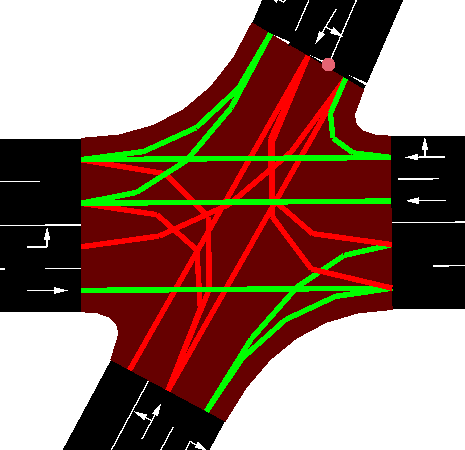
\includegraphics[width=.60\linewidth,valign=t]{my_folder/images//separate-state-0.png}
	\end{subfigure}
	\hfill %выровнять
	\adjustbox{minipage=1.3em,valign=t}{\subcaption{}\label{fig:state-b}}%
	\begin{subfigure}[t]{\dimexpr.3\linewidth-1.3em\relax}
		\centering
		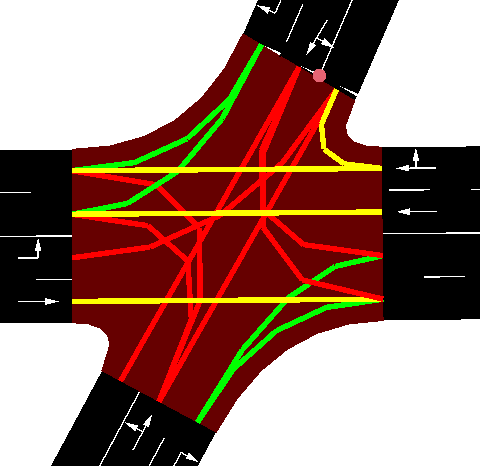
\includegraphics[width=.60\linewidth,valign=t]{my_folder/images//separate-state-1.png}
	\end{subfigure}
	\hfill %выровнять
		\adjustbox{minipage=1.3em,valign=t}{\subcaption{}\label{fig:state-c}}%
	\begin{subfigure}[t]{\dimexpr.3\linewidth-1.3em\relax}
		\centering
		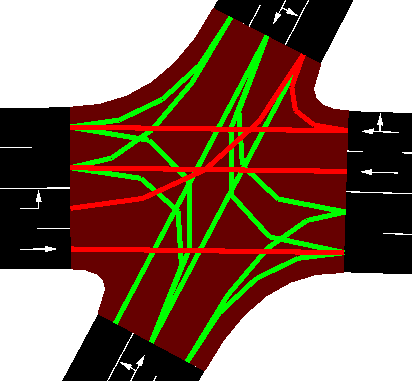
\includegraphics[width=.60\linewidth,valign=t]{my_folder/images//separate-state-2.png}
	\end{subfigure}%
\captionsetup{justification=centering} %центрировать
\caption{Пример смены состояний {\itshape a} $\rightarrow$ {\itshape b} $\rightarrow$ {\itshape c}}
\end{figure}




